% This template was initially provided by Dulip Withanage.
% Modifications for the database systems research group
% were made by Conny Junghans,  Jannik Strötgen and Michael Gertz

\documentclass[
     12pt,         % font size
     a4paper,      % paper format
     BCOR10mm,     % binding correction
     DIV14,        % stripe size for margin calculation
     ]{article}

%%%%%%%%%%%%%%%%%%%%%%%%%%%%%%%%%%%%%%%%%%%%%%%%%%%%%%%%%%%%

% PACKAGES:

% Use German
\usepackage[english]{babel}
% Input and font encoding
\usepackage[utf8]{inputenc}
\usepackage[T1]{fontenc}
% Index-generation
\usepackage{makeidx}
% Embedding of URLs
\usepackage{url}
% Special \LaTex symbols (e.g. \BibTeX)
%\usepackage{doc}
% Include Graphic-files
\usepackage{graphicx}
% Include doc++ generated tex-files
%\usepackage{docxx}
% Fuer anderthalbzeiligen Textsatz
\usepackage{setspace}
\usepackage[table,xcdraw]{xcolor}
\usepackage{hhline}
\usepackage{highlight}

\usepackage{subcaption}

\usepackage{biblatex}
\bibliography{references.bib}

% hyperrefs in the documents
\PassOptionsToPackage{hyphens}{url}\usepackage[bookmarks=true,colorlinks,pdfpagelabels,pdfstartview = FitH,bookmarksopen = true,bookmarksnumbered = true,linkcolor = black,plainpages = false,hypertexnames = false,citecolor = black,urlcolor=black]{hyperref}
%\usepackage{hyperref}


% CUSTOM:

% For Quotes:
\usepackage{csquotes}

% For Definitions:                   						
\usepackage{amsthm}
\usepackage[framemethod=tikz]{mdframed}

\newtheoremstyle{defi}
{\topsep}         % Abstand oben
{\topsep}         % Abstand unten
{\normalfont}     % Schrift des Bodys
{0pt}             % Einschub der ersten Zeile
{\bfseries}       % Darstellung von der Schrift in der �berschrift
{:}               % Trennzeichen zwischen �berschrift und Body
{.5em}            % Abstand nach dem Trennzeichen zum Body Text
{\thmname{#3}}    % Name in eckigen Klammern
\theoremstyle{defi}

\newmdtheoremenv[
hidealllines = true,       % Rahmen komplett ausblenden
leftline = true,           % Linie links einschalten
innertopmargin = 0pt,      % Abstand oben
innerbottommargin = 4pt,   % Abstand unten
innerrightmargin = 0pt,    % Abstand rechts
linewidth = 3pt,           % Linienbreite
linecolor = gray!40,       % Linienfarbe
]{defStrich}{Definition}     % Name der des formats "defStrich"

%For Abbreviations:
\usepackage{acronym}

%For Mathematical LaTeX Macros
\usepackage{mathtools}
\DeclarePairedDelimiter\abs{\lvert}{\rvert}%
\DeclarePairedDelimiter\norm{\lVert}{\rVert}%


%%%%%%%%%%%%%%%%%%%%%%%%%%%%%%%%%%%%%%%%%%%%%%%%%%%%%%%%%%%%

% OTHER SETTINGS:

% Choose language
\newcommand{\setlang}[1]{\selectlanguage{#1}\nonfrenchspacing}


\begin{document}

% TITLE:
\pagenumbering{roman} 
\begin{titlepage}

\vspace*{1cm}
\begin{center}
\textbf{ 
\Large Heidelberg University\\
\smallskip
\Large Institute of Computer Science\\
\smallskip
}

\vspace{3cm}

\textbf{\large Project report for the lecture Fundamentals of Machine Learning}

\vspace{0.5\baselineskip}
{\huge
\textbf{Reinforcement Learning for Bomberman}
}
\vspace{0.5cm}

\url{https://github.com/nilskre/bomberman_rl}

\end{center}

\vfill 

{\large
\begin{tabular}[l]{ll}
Team Member: & Felix Hausberger, 3661293,\\
  & Applied Computer Science\\
  & eb260@stud.uni-heidelberg.de\\
  & \\
Team Member: & Nils Krehl, 3664130,\\
  & Applied Computer Science\\
  & pu268@stud.uni-heidelberg.de\\
  
\end{tabular}
}

\end{titlepage}

\section*{Abstract}


\section*{Plagiarism statement}

We certify that this report is our own work, based on our personal study and/or research and that we have acknowledged all material and sources used in its preparation, whether they be books, articles, reports, lecture notes, and any other kind of document, electronic or personal communication.

We also certify that this report has not previously been submitted for assessment in any other unit, except where specific permission has been granted from all unit coordinators involved, or at any other time in this unit, and that we have not copied in part or whole or otherwise plagiarized the work of other students and/or persons.


\newpage
\tableofcontents
\newpage

\pagenumbering{arabic}

\section*{List of Abbreviations}

\begin{acronym}[WYSISWG]

	\acro{CUDA}{Compute Unified Device Architecture}
	\acro{DQN}{Deep-Q-Networks}
	\acro{ELU}{Exponential Linear Unit}
	\acro{MDP}{Markov Decision Process}
	\acro{ReLU}{Rectifier Linear Unit}
	\acro{PER}{Prioritized Experience Replay}

\end{acronym}
\section{Introduction}

Reinforcement Learning is a part of Machine Learning, where an agent is trained to interact in a desired way with its environment. Based on the current state, the agent decides for an action and can receive a reward for the chosen action. \cite{salvadorReinforcementLearningLiterature2020}

The potential of Reinforcement Learning is proven many times in varying contexts. E.g. attention was generated by the success of DeepMind's AlphaGo, the first artificial agent defeating a human in the game Go. For training this agent they used Reinforcement Learning. \cite{Silver1140}

Salvador, Oliveira and Breternitz have summarized the evolution of Rein\-force\-ment in a literature review \cite{salvadorReinforcementLearningLiterature2020}. They start in 1989 with the publication introducing Q-learning. In the recent past many publications deal with the combination of Deep Learning with Reinforcement Learning. This area is known as Deep Q-learning.

As part of this project we use Reinforcement Learning for learning how to play Bomberman. Bomberman is a strategic board game, which is played on a field containing walls, crates, bombs, coins and other players. For winning the game one must gather points by killing other players and collecting coins. Typically in each game round first the walls around the player are removed by placing bombs. Next the agent can navigate towards coins or towards his opponents and kill them by placing bombs. \cite{Kormelink2018}

After introducing the fundamentals and related work in chapter \ref{fundamentals_related_work}, our approach is described in chapter \ref{approach}. Therefore our selected Reinforcement Learning method and the training process are presented. In chapter \ref{experimental_results} the results of our experiments are described. A conclusion is drawn in chapter \ref{conclusion}.
\section{Fundamentals and Related Work} \label{fundamentals_related_work}

Q-Learning is a known off-policy and model-free approach to train an agent based on temporal difference in an environment that can be modeled as a Markov Decision Process (MDP). An agent therefore does not necessarily use the policy it is trained for and does not know the transition probabilities and rewards in the MDP beforehand. \autoref{QLearning} shows the interative update formula for the Q-values that an online model uses to choose the right action.

\begin{equation} \label{QLearning}
	Q_{k+1}(s,a) = (1-\alpha) Q_k(s,a) + \alpha(r + \gamma \max_{a'} Q_k(s',a')) 
\end{equation}

The problem with conventional Q-Learning is that in most of the cases the state dimension is far too high to explore and model the MDP entirely in foreseeable future. To deal with this problem the Q-values need to be approximated using a regression model. Deep neural networks have proven to be highly applicable for this task, which leads to the term of \textit{Deep-Q-Learning} and respectively \textit{Deep-Q-Networks} (DQN) for such network architectures. DQNs use the vectorized numerical state as its input and outputs the predicted Q-values. It learns through backpropagating the temporal difference error over each step. In the following papers regarding DQN architectures shall be introduced as well as papers dealing with the bomberman environment for reinforcement learning. 

Paper \cite{vanHasselt2015} introduces ...
\section{Approach} 
\label{approach}

\subsection{Reinforcement Learning Method and Regression Model} 
\label{ch:approachA}

% TODO: The first section shall describe the reinforcement learning method and regression model you finally implemented, including all crucial design choices. You may also describe approaches you tried and abandoned later, including the reasons.

\subsubsection{Features}
\label{ch:approachAa}

This chapter describes how the game state is transformed into input features for the model. 
Our initially tried encoding is based on \cite{Kormelink2018}. The dictionary containing the game state is transformed into one vector, containing the input features.
Our input feature vector consists of the following five independent matrices:
\begin{itemize}
	\item Field state: free (0), breakable (1), obstructed cell (0.5)
	\item Player position: player (1), otherwise(0)
	\item Opponent positions: opponent (1), otherwise(0)
	\item Danger level of position: danger (1), no danger (0) \newline
	Danger is caused by bombs on all fields an explosion can reach. Two aspects influence the value how dangerous a field is. The time until the bomb explodes and the distance from the bomb as escaping might become more difficult the closer an agent is to a bomb. We derived following equation for calculating the danger of a field for the field containing the bomb and the surrounding fields. The resulting danger score is normalized through the equation in the range between 0 and 1.
	
	$ danger = \frac{\frac{time\_Passed}{time\_needed\_to\_explode}}{\sqrt{distance}} $
	
	Example 1: the bomb explodes after 4 time steps. Currently 2 time steps are over and the distance to the bomb is 3:
	
	$ danger = \frac{\frac{2}{4}}{\sqrt{3}} = 0.28 $
	
	Example 2: the bomb explodes after 4 time steps. Currently 3 time steps are over and the distance to the bomb is 1:
	
	$ danger = \frac{\frac{3}{4}}{\sqrt{2}} = 0.75 $
	
	\item Desirability of position: coin (1), no coin (0)
\end{itemize}
These matrices are flattened and concatenated. This results in a feature vector containing 1445 elements (5*17*17).

Among other factors due to the high dimensionality the training process could be very slow. That is why the input state is further minimized.
Franca, Paes and Clua \cite{Franca2019} evaluated five different strategies for state representation (Binary Flag, Normalized Binary Flag, Hybrid, ICAART, ZeroOrOne). The performance of the different encodings is measured by the cumulative rewards during training in relation to the number of episodes. Their results were that Hybrid, ICAART and ZeroOrOne perform better than Binary Flag and Normalized Binary Flag. The best encoding regarding to \cite{Franca2019} is ICAART. That is why our finally implemented encoding is based on ICAART.

The following paragraphs describe our finally chosen encoding:
The matrices above encode three different types of information:
general information (field state, player position, opponent positions), desired positions (Desirability of position) and dangerous positions (Danger level of position).
We minimize the input state by concatenating general information and desired positions in one matrix and dangerous fields in another one. This keeps the balance between clearly separated information and maximal state minimization.

\begin{itemize}
	\item General information and desired positions: free (0), breakable (1.5), obstructed cell (-1.5), own position (2), opponent positions (-2), coin (1)
	\item Danger level of position: danger (-1), no danger (0)
\end{itemize}
These matrices are flattened and concatenated. This results in a feature vector containing 578 elements (2*17*17).

As further optimization one could also include behavioral information as part of the features. E.g. one could encode the optimal path towards the coins as one feature or reactions after placing a bomb (run away) as another feature. Such a feature representation could be interpreted as step away from a machine learning based agent towards a rule-based agent as the task of learning the optimal movement was already encoded inside the feature space. In order to avoid this gray area of potentially violating the project guidelines it was decided to not implement feature representations, which enhance the state information by behavioral information.

\subsubsection{Dueling Double Deep Q-Network}
\label{ch:approachAb}

Based on the literature research, described in chapter \ref{fundamentals_related_work}, a dueling double DQN approach was selected. The concrete implementation and structure of this approach can be seen in figure \ref{fig:model}.
In the first layer, our feature vector (chapter \ref{ch:approachAa}) is inserted. The input layer is followed by a fully connected Dense layer. In the next step the dueling optimization is implemented. By the Lambda layer the input is split into a value and an advantage stream. 
The advantage stream consists of a Flatten layer, a Dense layer and a custom Lambda layer for reducing the mean.
The value stream is first flattened by a Flatten layer and then fed into a fully connected Dense layer.
Finally both streams are again merged for receiving the final Q values.

\begin{figure}[ht]
	\centering
	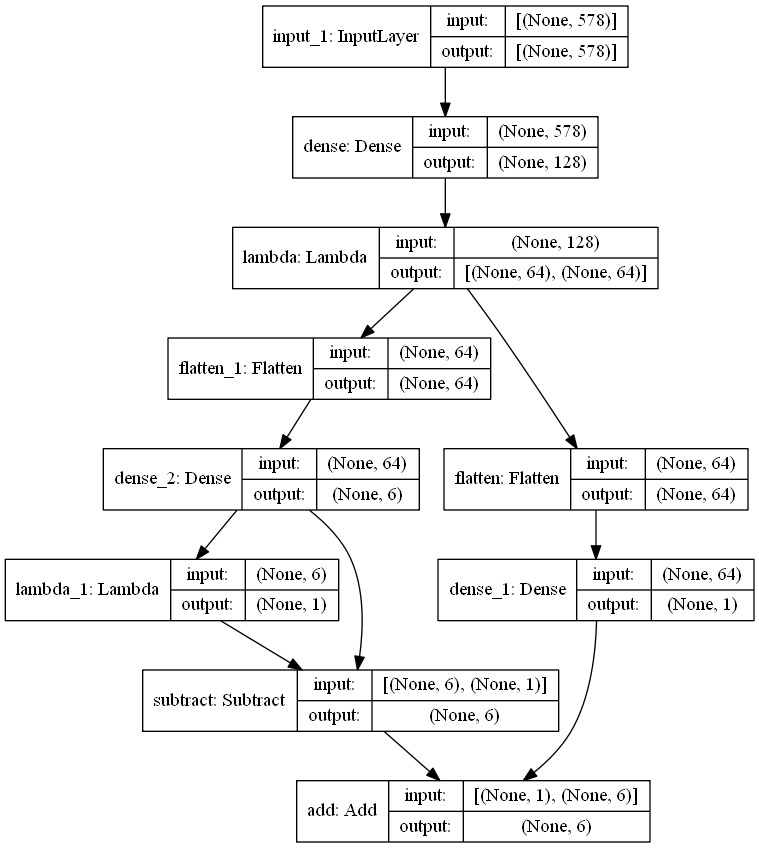
\includegraphics[width=0.8\linewidth]{figures/model.jpeg}
	\caption{Structure of the DQN model}
	\label{fig:model}
\end{figure}

\subsection{Training process} 
\label{ch:approachB}

% TODO: The second section should describe your training process, including all tricks employed to speed it up (e.g. self play strategy, design of auxilliary rewards, prioritization of experience replay and so on).

\subsubsection{Exploration-Exploitation}
\label{ch:approachBa}

When choosing the right method for the exploration-exploitation tradeoff, \cite{Kormelink2018} gives an insight in how different exploration methods perform in the Bomberman environment (see \autoref{fig:exploration}). 

\begin{figure}[ht]
	\centering
	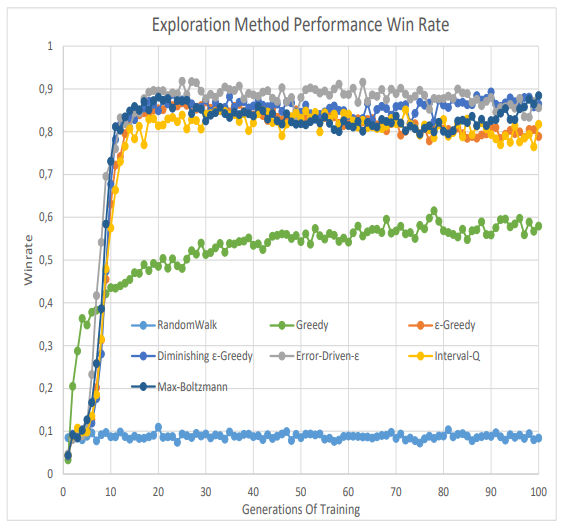
\includegraphics[width=0.6\linewidth]{figures/exploration.PNG}
	\caption{Comparison of different exploration methods}
	\label{fig:exploration}
	\cite{Kormelink2018}
\end{figure}

In the long run, Max Boltzmann performs best with 

\begin{equation}
	\Pi(s,a) = \frac{e^{Q(s,a)/T}}{\sum_i^{\abs{A}}e^{Q(s,a^i)/T}}
\end{equation}

and T being the temperature parameter. But as the result is based on 100 generations of training with each generation comprising 10.000 episodes, Diminishing $\epsilon$-Greedy as the second best exploration method was chosen as this exploration method converges faster in the early stages of training.

Two improvements where considered to optimize the exploration phase, but were discarded in the end. The first one is to replace the uniform sampling method by a multinomial sampling method in case an exploration step should be done, i.e. when a randomly generated number is smaller than $\epsilon$. This means the second best action would be chosen more often compared to other actions during the exploration phase. This could be beneficial especially in later phases of training in case the Q-values are close to each other. But esspecially in the beginning of the training phase this could lead towards an unintended bias towards specific actions as the exploration of others will be suppressed probabilistically.

The second improvement was to include an exploration function as \cite{Geron2018} proposes. A simple exploration function could be 

\begin{equation}
	f(q,n) = q + \frac{K}{1+n}
\end{equation}

with $q$ being the Q-value and $n$ being the count how often a specific action $a$ was chosen in state $s$. $K$ is a hyperparameter that determines the amount of curiosity during training. To implement this one would need to store $n$ for every state and action. But as the state is far too high dimensional in the Bomberman environment this would require a lot of training just as using the Max Boltzmann exploration method to be beneficial in the end. 

\subsubsection{Prioritized Experience Replay Buffer and SumTree}
\label{ch:approachBb}

Furthermore, a prioritized experience replay buffer was utilized to speed up the training process. To efficiently sample from it, a SumTree data structure was implemented inspired by \cite{Schaul2016}, which is a binary tree whose parent nodes store the sum of its children. All leaf nodes of the SumTree store the priority of each temporal difference error which is the L1-norm between two succeeding Q-values. The SumTree inherently offers a stratified sampling method to sample experiences with a high temporal difference error and therefore high priority more often. Therefore the leaf nodes are grouped into sum segments with a sum value greater or equal a threshold value. Each segment can therefore contain a different amount of leaf nodes as priorities often differ in their magnitude. The amount of segments is determined by the demanded batch size and the threshold value by dividing the total sum of the tree (stored in the root node) by the batch size. From each segment one priority is sampled uniformly. As high priorities have less competitors in their segment, they will be sampled more frequently until they get overwritten.  

\begin{figure}[ht]
	\centering
	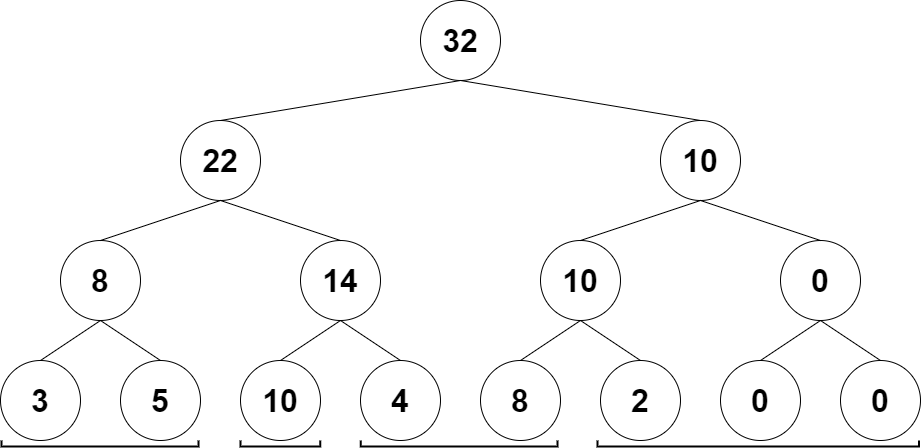
\includegraphics[width=0.6\linewidth]{figures/sumtree.PNG}
	\caption{Stratified sampling of priorities from a SumTree}
	\label{fig:sumtree}
\end{figure}

\autoref{fig:sumtree} illustrates the process of sampling priorities with a batch size of four. One can see that the priority with magnitude ten will be sampled every time as it is the only priority within the sum segment. One can also see that in case the prioritized experience replay buffer is not filled, zeros might be sampled. To counteract this, the amount of sum segments to divide the SumTree into is the batch size plus one. Adding values to the SumTree has the complexity O(1) whereas subsequent updating the SumTree has the complexity O(log n). 

The prioritized experience replay buffer only stores the priorities in the SumTree. The tuple $(s,a,r,s')$ is stored in a separate list. To access the according experience tuple for a priority, one can easily calculate the acording index by $index_{list} = index_{tree} - size_{per} + 1$. Note that \autoref{prio2} is used to calculate the priority value for each temporal difference error instead of \autoref{prio} as one would need to also sort the priorities in a different data structure which would add additional complexity and computing time. When sampling a batch from the prioritized experience replay buffer the tupel $(s,a,r,s')$, the according priorities, normalized weighting factors and update indices are returned. 

Drawbacks of using a prioritized experience replay buffer over a normal experience replay buffer is the continuous maintenance of the SumTree data structure, which is currently updated every training step, i.e. every step in an episode. Updated value changes need to be propagated to the root node. This adds additional computing time but the time gained in training progress by using prioritization should make up the time lost by maintaining the SumTree. Besides updating existing experiences every step also a new experience is added to the prioritized experience replay buffer every step which on the other hand executes fast. 

\subsubsection{Imitation Learning}
\label{ch:approachBc}

For addressing the challenge of long training times, Imitation Learning can be used. With the rule-based agent, already a strong agent is present in the project. The idea of Imitation Learning is to speed up training by learning from existing behavior (e.g. from the rule-based agent).

The general applicability of Imitation Learning was evaluated by Hester et al. \cite{hester2017deep} and the application of Imitation Learning for the game Bomberman was examined by Franca, Paes and Clua \cite{Franca2019}.

Hester et al. \cite{hester2017deep} stated, that their Imitation Learning approach (Deep Q-learning from demonstrations) is better then a prioritized dueling double Deep Q-Network approach. Furthermore they have discovered, that the trained agent is able to outperform the behavior shown in training.

Franca, Paes and Clua \cite{Franca2019} have found out in a setting comparable to our project that Imitation Learning followed by Proximal Policy Optimization (PPO) Learning achieves the best results. The PPO algorithm is a model-free Reinforcement Learning algorithm, which uses the advantage operator instead of Q-values.

As optimization for our approach (chapter \ref{ch:approachAb}), we implemented Imitation Learning based on \cite{hester2017deep}. This optimization is realized by splitting the training into a pretraining phase and a training phase. In the pretraining phase the Imitation Learning takes place. The experience replay buffer is filled by the actions of the rule-based agent and the DQN is pretrained.
In the training phase the standard Reinforcement Learning approach takes place. Based on the pretrained DQN and the filled experience replay buffer the training process is executed. For an evaluation of this training structure please refer to \autoref{experimental_results}.

\subsubsection{Reward Shaping}
\label{ch:approachBd}

Rewards are given when different kind of actions are taken or different kind of events occur. An overview of all rewards is given in \autoref{tab:rewards}.

\begin{table}[hbt!]
	\caption{Reward function}
	\label{tab:rewards}
	\begin{tabular}{|p{0.6\textwidth}|p{0.3\textwidth}|}
		\hline
		\textbf{Reward} & \textbf{Amount} \\ \hline
		Movement in/out of danger zone & -0.3/+0.3 \\ \hline
		Movement towards/away from nearest coin & +0.1/-0.1 \\ \hline
		Movement towards/away from nearest opponent & +0.05/-0.05 \\ \hline
		WAITED & -0.2 \\ \hline
		INVALID\_ACTION & -1 \\ \hline
		BOMB\_DROPPED & 0.4 \\ \hline
		CRATE\_DESTROYED & 0.7 \\ \hline
		COIN\_COLLECTED & 0.2 \\ \hline
		KILLED\_OPPONENT & 1 \\ \hline
		KILLED\_SELF & -1 \\ \hline
		GOT\_KILLED & -1 \\ \hline
	\end{tabular}
\end{table}

Setting the rewards properly is a very difficult task and hard to evaluate without empirical study. Specifically for the Bomberman environment only few literatue was found that covers a reward function \cite{Kormelink2018, Franca2019}. All rewards are normalized to be in between -1 and 1 for more efficient training. Also focus was set on giving reward feedback as soon as possible to guide the training process better towards the desired behavior. 

In the first step the agent should be encouraged to gather coins, which is why the movement towards the nearest coin is rewarded. Nevertheless especially in the beginning of a game and also in late game phases setting bombs to find coins, to explore the arena and to kill opponents is even more crucial than finding coins. This is why the reward for dropping bombs is even higher than moving towards coins and gathering coins. To place bombs near creates the reward for destroying crates is set above the reward to simply dropping a bomb. 

Having this setup of arranging rewards leads to a lot of suicide of the agent in the very beginning of the training phase even if the the own agents death is punished. Therefore rewards for moving out of danger zones and punishments for moving in danger zones are given to encourage the agent to walk away from bombs dropped. Note that this reward is even higher than the movement reward towards the nearest coin to keep an agent out of a danger zone in case a coin is located in the bomb radius. 

Also an agent doing nothing or a invalid action should be punished by a negative reward. Therefore also no reward is given for rounds survived. Committing suicide or idleing was a big problem especially in the early stages of the training phase that should be countered using the introduced reward function. 

Killing opponents gives the highest reward, which is exactly five times higher than collecting a coin just like the points given inside the game. Finally to encourage an agent to also move towards an opponent agent an additional movement reward is given for moving towards the nearest opponents and a punishment in case the agent runs away from the nearest agent. Nevertheless such a reward is scaled quite low and only becomes more important in the late game steps. In the early stages of a game the agent should rather learn how to collect coins, how to destroy crates and how to survive. 

One could also think of introducing a reward schedule that increases certain rewards during a game and lowers others. This could be applied when all coins are collected and an agents score can only be increased by killing opponents. Such a dynamic adjusting reward function still has to be evaluated.

\subsubsection{Hyperparameters}
\label{ch:approachBe}

\autoref{tab:hyperparameters} shows the choice of hyperparameters during training. As the computing resources are limited the hyperparameters were chosen to reach a fast convergence towards a first proper behavior which does not need to be optimal in the first place. \cite{Kormelink2018} states to train an agent over 100 generations à 10.000 episodes whereas the win rate in \autoref{fig:exploration} is already quite high just after 10 generations. Having 400 steps per episode one generation can be trained locally within six hours which is really low inspite of using CUDA on a graphics card with a computing power score of 6.1 of 10. For further information one the local setup please refer to \autoref{ch:approachBg}. Note that the hyperparameters in \autoref{tab:hyperparameters} are the ones initially chosen, they were further adapted during the experimental phase in \autoref{experimental_results}.

\begin{table}[hbt!]
	\caption{Hyperparameters}
	\label{tab:hyperparameters}
	\begin{tabular}{|p{0.6\textwidth}|p{0.3\textwidth}|}
		\hline
		\textbf{Hyperparameter} & \textbf{Value} \\ \hline
		Dense layer dimension & 128 \\ \hline
		\hline
		Activation function & ELU \\ \hline
		Loss function & Huber \\ \hline
		Learning rate & 0.01 \\ \hline
		\hline
		$\alpha$ & 0.65 \\ \hline
		$\beta$ & 0.4 \\ \hline
		$\beta$ increment & 0.00001 \\ \hline
		temporal difference $\epsilon$ bias & 0.01 \\ \hline
		\hline
		PER buffer min size & 8.192 \\ \hline
		PER buffer max size & 65.536 \\ \hline
		Batch size & 64 \\ \hline
		\hline
		$\gamma$ & 0.95 \\ \hline
		$\epsilon$ start & 0.3 \\ \hline
		$\epsilon$ end & 0.16 \\ \hline
		$\epsilon$ decay factor & 0.99999 \\ \hline
	\end{tabular}
\end{table}

The amount neurons per dense layer inside the dueling double DQN should not be higher than the input dimension itself as such a high degree of freedom is not needed to model the bomberman environment. For simplicity of the training process 128 was prefered over 256. 

The Exponential Linear Unit (ELU) activation function was chosen to fight the dead ReLU problem and to speed up training by pushing the mean activation towards zero and therefore decreasing the bias shift from ReLU. To be more robust towards outliers a Huber loss function was prefered over a conventional Squared Error loss function. The learning rate was set quite high with 0.01 to reach a fast convergence towards a first playable behavior on limited computing resources. 

The choice of the prioritized experience replay buffer hyperparameters was inspired by \cite{Schaul2016}. $\alpha$ was chosen slightly higher to once again speed up training through more prioritization. The $\beta$ increment summand was chosen just as high to converge $\beta$ to 1 at approximately the same time as $\epsilon$ converges to its lower limit after around 60.000 steps. 

The size of the prioritized experience replay buffer needs to be a power of two to result in a balanced SumTree. The batch size should be lower than one percent of the total prioritized experience replay buffer size, which is why the minimum size of the prioritized experience replay buffer was chosen to be 8192. This leads to a start of the training process after around 21 episodes. 

Choosing the right $\gamma$ in approximative Q-learning is not too important as future rewards are approximated. Using a decaying factor of $\gamma=0.95$ means rewards after 13 steps are only half that important as current rewards. $\epsilon$ is often decayed to around 0.05-0.2 and starts at either 1 or 0.3 \cite{Hessel2017, Kormelink2018, Franca2019}. As Imitation Learning in the pre-training phase already gives a good first behavioral model and also to not have too much random behavior in the beginning 0.3 was chosen as the start value for $\epsilon$. 

Furthermore, the model and the  prioritized experience replay buffer are stored every 100 epsiodes in case the training process crashes because of unforeseen events. 

\subsubsection{Cloud Training}
\label{ch:approachBf}

To further accelerate the training process and enable fast iterations for im\-pro\-ving the approach in reasonable feedback loops, the possibility of training in the cloud was evaluated. 

The prospects of success were shown by Lawrence et al. \cite{Lawrence2017ComparingTD}. They evaluated the TensorFlow Deep Learning performance between CPUs, GPUs, local computers and the cloud. Their findings were that the usage of GPUs leads to a significant performance increase. Furthermore the cloud is not better by default. That is why it is recommended to compare the GPU performance metrics (e.g. compute capability score) of the local and the cloud configuration. The following table \ref{table:hardware} compares common GPUs.
Especially Nvidia is known in the area of GPUs for it's Compute Unified Device Ar\-chi\-tec\-tu\-re (CUDA). It provides a programming model and parallel computing platform for outsourcing processes to the GPU. In the area of Deep Learning there is the supplementary library called Nvidia CUDA Deep Neural Network Library (cuDNN), which provides hardware optimized routines for Deep Learning tasks.

\begin{center}
	\begin{tabular}[H]{l|c|c|c|c|c|c}
		& K80 & P100 & T4 & V100 & GTX 1080 \\
		\hline
		CUDA Cores & 2496 & 3584 & 2560 & 5120 & 2560 \\
		Tensor Cores & / & / & 320 & 640 & / \\
		TeraFLOPS (Single Precision) & 4,113 & 9,526 & 8,141 & 14,13 & 9,784  \\
		Memory Bandwidth (GB/sec) & 240,6 & 732,2 & 320 & 897 & 345,6 \\
		Suggested Power Supply Unit & 700 & 600 & 350 & 600 & 450 \\
		Compute capability & 3.7 & 6.0 & 7.5 & 7.0 & 6.1 \\ 
	\end{tabular}
	\captionof{table}{GPU comparison}
	\label{table:hardware}
	Based on \cite{techpowerupeditorTechPowerUp} and \cite{nvidiaeditorCUDAGPUs2012}
\end{center}


Based on these basic information regarding training hardware and the associated findings, for our purposes two requirements exist:
\begin{enumerate}
	\item The Cloud GPUs should be much more performant than the local GPU (local GPU: GTX 1080). To notice visible improvements we at least expect a compute capability score of seven.
	\item The GPUs could be used for free.
\end{enumerate}

Hale \cite{haleBestDealsDeep2019} compares the following Cloud providers: Google Colab, Google Cloud Platform, AWS, Paperspace and vast.ai. In general either the first or the second requirement are not fulfilled by the different cloud providers. 

This is exemplary illustrated by means of Google Colab and Google Cloud Platform. 
On the one hand Google Colab can be used after converting the project into one Jupyter Notebook. GPUs can be used for a limited time frame for free. The available GPUs are Nvidia K80s, T4s, P4s and P100s, which are assigned automatically \cite{googleeditorColaboratoryGoogleFAQ}. The compute capability score lies depending on the GPU between 3.7 and 7.5 \cite{nvidiaeditorCUDAGPUs2012}. So Google Colab matches the second requirement, but not necessarily the first one. Also much effort would have had to be invested into converting the project into a Jupyter Notebook. 
On the other hand the Google Cloud Platform, especially the AI Platform offers many performant GPUs to choose from, but it can quickly become very expensive, as the following example calculation shows \cite{googleeditorGPUsTrainierenModellen}. 

The calculation was done with the Google Cloud Pricing Calculator \cite{googleeditorGoogleCloudPlatformPreisrechner} and following parameters:
\begin{itemize}
	\item Region: United States
	\item Selected tier: BASIC\_GPU
	\item Job run time in minutes: 4320min (3 days)
	\item => estimated costs: 71.93€
\end{itemize}

That is why the Google Cloud Platform matches the first requirement, but not the second one.

Based on the above findings the possibility of cloud training is not realized and the training process is executed locally. 

\subsubsection{Local Training Setup}
\label{ch:approachBg}

As mentioned in the previous chapter our local training setup is based on the GPU Nvidia GTX 1080 with a comuting power of 6.1 out of 10. Furthermore we use CUDA (version 11.2.1) and the cuDNN library (version 8.1.0). In cooperation with TensorFlow (version 2.4.1) it is ensured that the local hardware is used optimally for the training process. The performance during training heavily depends on the progress a model has made so far. Pre-training usually takes longer as the full 400 steps are normally taken per episode which results in a performance of 1000 episodes in nine hours. At the beginning of the main training phase, esspecially when the amount of exploration is still high and the model did not converge yet, 1000 episodes can trained in less then one hour (approx. 35 minutes).  

\subsubsection{Training Visualization}
\label{ch:approachBh}




\section{Experimental results} \label{experimental_results}

% TODO: The third section shall report experimental results (e.g. training progress diagrams), describe interesting observations, and discuss the difficulties you faced and how you overcame them.

When starting the initial training process first a pre-training is executed which serves to fill the prioritized experience replay buffer with experiences from an expert rule-based agent and to pre-train the model itself to build up on some agent behavior already for the later training process. To not introduce a heavy bias the pre-training is stopped after 1.500 training games. \autoref{fig:pre-loss-1} shows the aggregated step loss per episode averaged after five episodes and \autoref{fig:pre-reward-1} the reward per episode averaged after five episodes.

\begin{figure}[ht]
	\centering
	\begin{subfigure}[b]{0.49\textwidth}
		\centering
		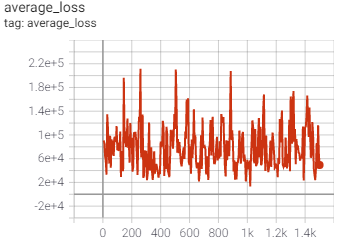
\includegraphics[width=\textwidth]{figures/training1-pre-loss.PNG}
		\caption{Pre-training loss}
		\label{fig:pre-loss-1}
	\end{subfigure}
	\hfill
	\begin{subfigure}[b]{0.49\textwidth}
		\centering
		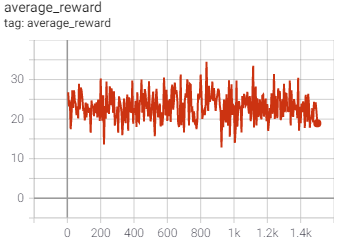
\includegraphics[width=\textwidth]{figures/training1-pre-reward.PNG}
		\caption{Pre-training average reward}
		\label{fig:pre-reward-1}
	\end{subfigure}
\end{figure}

The two charts are not too surprising, the reward should on average be the same with a rule-based behavior. Also the loss does not decrease much with only 1.500 episodes of pre-training. When initiating the main training process with experiences gained from the dueling double DQN itself the following training curves can be experienced:

\begin{figure}[ht]
	\centering
	\begin{subfigure}[b]{0.49\textwidth}
		\centering
		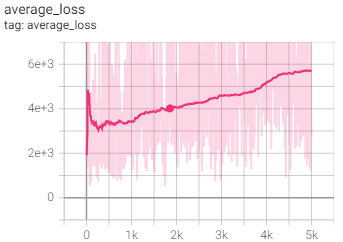
\includegraphics[width=\textwidth]{figures/training1-main-loss-smooth.PNG}
		\caption{Main-training loss}
		\label{fig:main-loss-smoothed-1}
	\end{subfigure}
	\hfill
	\begin{subfigure}[b]{0.49\textwidth}
		\centering
		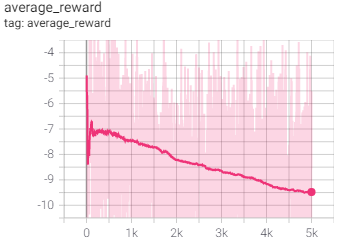
\includegraphics[width=\textwidth]{figures/training1-main-reward-smooth.PNG}
		\caption{Main-training average reward}
		\label{fig:main-reward-smoothed-1}
	\end{subfigure}
\end{figure}

The complete opposite of what was expected was observed, the loss increased whereas the average reward decreased. One possible explanation was a possible training bias introduced through the prioritized experience replay buffer towards transition with a high temporal difference error. Even if the gradient weighting factors were calculated and used to anneal the bias as proposed in the original paper, still this unintended behavior could be experienced. Therefore the training process was aborted after 5.000 episodes. 

The next generation of the model was trained on a normal experience replay buffer with the following results:

\begin{figure}[ht]
	\centering
	\begin{subfigure}[b]{0.49\textwidth}
		\centering
		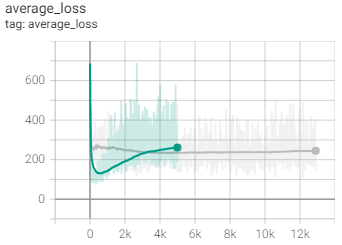
\includegraphics[width=\textwidth]{figures/training2-main-loss-smooth.PNG}
		\caption{Main-training loss}
		\label{fig:main-loss-smoothed-2}
	\end{subfigure}
	\hfill
	\begin{subfigure}[b]{0.49\textwidth}
		\centering
		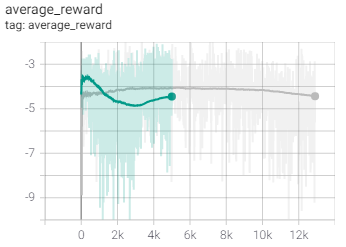
\includegraphics[width=\textwidth]{figures/training2-main-reward-smooth.PNG}
		\caption{Main-training average reward}
		\label{fig:main-reward-smoothed-2}
	\end{subfigure}
\end{figure}

Also, the initial exploration factor $\epsilon$ was increased from 0.3 to 1 to counter a possible pre-training bias and the maximum size of the experience replay buffer was decreased from 65.536 to 32.768 to train on more recent experiences. The green curve shows the training development until 5.000 episodes, which was then expanded to another 13.000 episodes plotted in the gray curve. 

Having done these changes results in a far lower training loss curve which converges to an average episode loss of 250 per five episodes. Also the reward curve seems to converge at an average loss of about minus four. Nevertheless, this average reward still is not what was expected and when looking at the actual agent behavior, the agent always chooses to wait. A possible explanation for this might be that the agent tries to avoid future punishments by just waiting until it gets killed by another player. 

To escape the bad local optimum and the small degree between rewards and punishments, the reward function was first slightly adjusted by increasing the magnitue of each reward by 100 and therefore breaking the normalization. This results in the two following training curves:

\newpage

\begin{figure}[ht]
	\centering
	\begin{subfigure}[b]{0.49\textwidth}
		\centering
		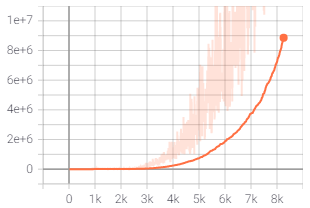
\includegraphics[width=\textwidth]{figures/training3-main-loss-smooth.PNG}
		\caption{Main-training loss}
		\label{fig:main-loss-smoothed-3}
	\end{subfigure}
	\hfill
	\begin{subfigure}[b]{0.49\textwidth}
		\centering
		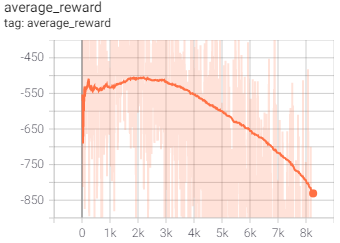
\includegraphics[width=\textwidth]{figures/training3-main-reward-smooth.PNG}
		\caption{Main-training average reward}
		\label{fig:main-reward-smoothed-3}
	\end{subfigure}
\end{figure}

As one can see this negatively impacts the training behavior exponentially and got discarded right away. In the next try the adaption of the rewards were discarded again, the exploration factor $\epsilon$ remained at a start value of one and the maximum size of the experience replay buffer was left at 32.768. The amount of episodes to train during the main training was increased to 30.000. This equals three generations which should show at least some improvements during the training process as in \cite{Kormelink2018} (see \autoref{fig:exploration}), especially when increasing the exploration. The following training curves were experienced: 

\begin{figure}[ht]
	\centering
	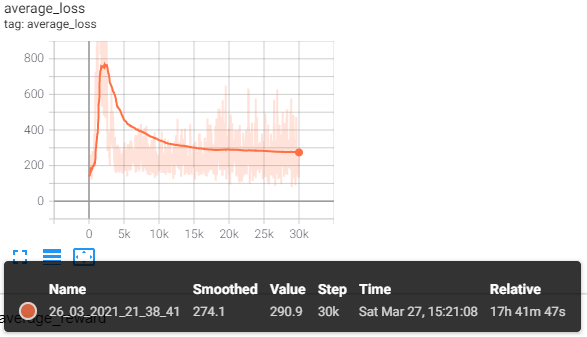
\includegraphics[width=0.8\textwidth]{figures/training4-main-loss-smooth.PNG}
	\caption{Main-training loss}
	\label{fig:main-loss-smoothed-4}
\end{figure}

When looking at the smoothed loss (see \autoref{fig:main-loss-smoothed-4}) one can see the curve falls strictly monotonously from 1.155 after around 2.000 episodes to 291 after 30.000 episodes. Having this setup taking the loss to around zero would still take ages when training locally. One could increase the learning rate, but previous experiments showed that this highly destabilized the training as the learning rate with 0.01 is already quite high compared to other papers \cite{Franca2019, Kormelink2018}. 

\begin{figure}[ht]
	\centering
	\begin{subfigure}[b]{0.49\textwidth}
		\centering
		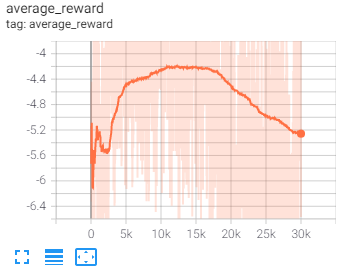
\includegraphics[width=\textwidth]{figures/training4-main-reward-smooth.PNG}
		\caption{Main-training average reward}
		\label{fig:main-reward-smoothed-4}
	\end{subfigure}
	\hfill
	\begin{subfigure}[b]{0.49\textwidth}
		\centering
		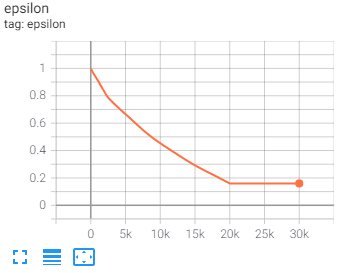
\includegraphics[width=\textwidth]{figures/training4-epsilon.PNG}
		\caption{$\epsilon$-decay}
		\label{fig:epsilon-4}
	\end{subfigure}
\end{figure}

Having higher exploration did not fix the problem of ecaping the bad local optimum of the agent waiting until it gets killed. Instead it just seems to extend the training process as the loss is even higher than before. The course of the average reward curve (see \autoref{fig:main-reward-smoothed-4}) equals to the original one, but now after 18k episodes the average reward curve falls again. This development also seems to be independent from the exploration rate development (see \autoref{fig:epsilon-4}) that now reaches its lower bound far later after 20.000 episodes. 

To summarize neither changing the magnitude of the rewards, nor increasing the exploration rate helped to escape the bad local optimum. Only increasing the training episodes seems to very slowly decrease the loss which might result in another optimum in the future as one would expect when looking at \autoref{fig:exploration}. The 30.000 episode training mark was reached after 17,67 hours which means another approx. 41 hour training to reach the 10 generations mark. As such a training takes its time and does not guarantee its success, it was decided to not pursue this further in the given amount of time. 

\newpage

\section{Conclusion} \label{conclusion}

% TODO: The final section shall give an outlook on how you would improve your agent if you had more time, and how we can improve the game setup for next year.

Unquestionably, there is a lot of research provided in the field of Deep Q-learning achieving impressive results. Unfortunately, much less research is provided in common problems when facing Reinforcement Learning issues, instead the same problems are re-discovered over and over again. A. Irpan, software engineer at Google Brain, summarizes these problems to point research into a common direction \cite{Irpan2018}. Some of the problems described match with the ones met within this project.

One of them is the difficulty to design a reward function that matches the given environment and domain exactly right. Otherwise shaped rewards might introduce a bias that overfits to certain actions. This was experienced as the agent overfits to waiting as to avoid future punishments. 

Even when having a well designed reward function, still it might be difficult to escape a local optimum. This phenomenon originates in a bad exploration-exploitation trade-off with much exploration leading to misleading data and bad training results and much exploitation leading to burn-in behaviors. This could be tackled by using count-based or curiosity-driven exploration as introduced in \autoref{expfunc}. Once again the behavior of the agent was also tried to be explained with this context. The bad local optimum was tried to escape by increasing the initial exploration rate $\epsilon$ while using the diminishing $\epsilon$-greedy exploration method. 

Even after a successful training one could not guarantee that the agent would have behaved the same way as during training. Especially when training against a certain other model these models could tend towards a co-evolution during training that makes them generalize weakly when being put into another environment. 

To conclude the difficulties faced during training the agent using a dueling double DQN, one can conclude: 

\begin{quote}
	\textit{\grqq[...] RL is very sensitive to both your initialization and to the dynamics of your training process, because your data is always collected online and the only supervision you get is a single scalar for reward. [...]. A policy that fails to discover good training examples in time will collapse towards learning nothing at all, as it becomes more confident that any deviation it tries will fail.\grqq} \cite{Irpan2018}
\end{quote}

Several improvements for future versions of the agent were collected. First the feature vector could be restricted to behavioral features instead of pure state features, which means pre-calculating certain tasks and only encode movement information and special game fields as features. This simplifies the learning process by not only minimizing the feature dimension but also by increasing the entropy of the features and therefore the degree of learning capability. Another way to alternate the feature vector is to use the actual encoded image of the playing field and giving it to a preceding convolutional neural network that is capable of recognizing certain patterns. Therefore similarities between states could be recognized and be encoded as the same feature vector that is then given to the normal dueling double DQN. This could once again minimize the feature space to important features only and therefore speed up the training process. 

Next the reward function could be extended by dynamically adjusting certain rewards during the progress of a game like increasing the movement reward towards opponents. This has not become important so far as the agent does not reach the late game phase in the original environment. 

This could be accomplished by utilizing count-based or curiosity-driven exploration to achieve a better exploration-exploitation trade-off or by pursueing more empirical experiments with different reward functions to escape the bad local optimum. 

Last but not least, the episodes to train could be increased to evaluate whether the loss in \autoref{fig:main-loss-smoothed-4} would converge to zero and the reward in \autoref{fig:main-reward-smoothed-4} would actually start to increase again and therefore escape the bad local optimum of the agent always waiting. 





\clearpage
\pagenumbering{Roman}
\appendix
\section{Appendix}

\subsection{Appendix A}
\label{ch:app-A}

tbd

%%%%%%%%%%%%%%%%%%%%%%%%%%%%%%%%%%%%%%%%%%%%%%%%%%%%%%%%%%%%

\newpage
\printbibliography

\end{document}
